\section{Neural Networks}

\begin{mdframed}
    \textbf{Neural Networks:} model inspired by the structure and function of biological neural networks in animal brains.
\end{mdframed}

\subsection{Architecture}
Architecture in the context of neural networks refers to the pattern developed to connect different neurons together.  Typically, neurons are organized by levels (layers).  In this course, only fully connected architectures are addressed, that is, where all neurons in one layer are connected to those in the next layer.
\begin{center}
    \begin{tabular}{c}
        \\ 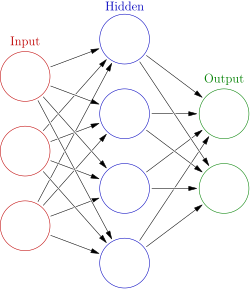
\includegraphics[width=0.35\textwidth]{images/NeuralNetworks1.png} \\ \\
    \end{tabular}
\end{center}
In this example a 2 layer neural network is schematized, one of which is hidden, for the nomenclature we do not consider the input layer since it is not affected by the parameters.  When going to establish the architecture of a neural network one goes to establish the number of parameters to be learned.
\begin{center}
    \begin{tabular}{c}
        \\ 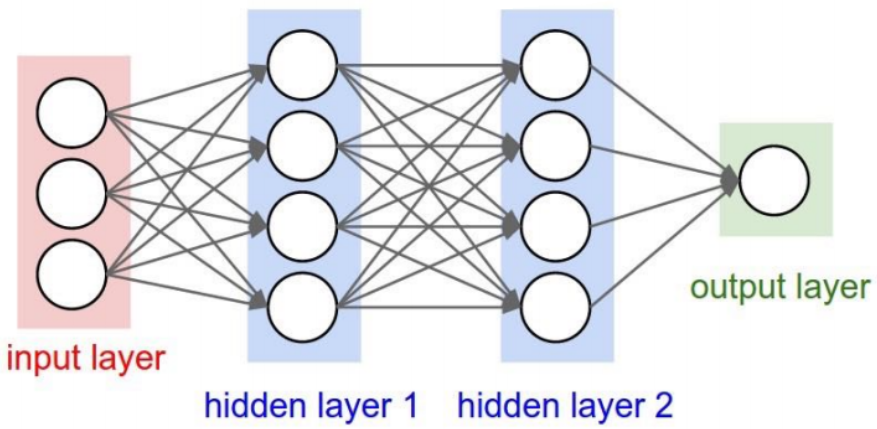
\includegraphics[width=0.6\textwidth]{images/NeuralNetworks2.png} \\ \\
    \end{tabular}
\end{center}
The total number of parameters is given by the sum of:
\begin{itemize}
    \item $3$ (\# neurons \textcolor{red}{input layer}) $\times 4$ (\# neurons \textcolor{blue}{hidden layer 1})
    \item $4$ (\# neurons \textcolor{blue}{hidden layer 1}) $\times 4$ (\# neurons \textcolor{blue}{hidden layer 2})
    \item $4$ (\# neurons \textcolor{blue}{hidden layer 2}) $\times 1$ (\# neurons \textcolor{green}{output layer})
    \item $4$ (bias \textcolor{blue}{hidden layer 1})
    \item $4$ (bias \textcolor{blue}{hidden layer 2})
    \item $1$ (bias \textcolor{green}{output layer})
\end{itemize}

\subsection{Feed-Forward Computation}
\begin{mdframed}
    \textbf{Feed-Forward:} neural networks in which the outputs of one layer become the inputs of the next layer.   Each output will be the weighted sum of the inputs of the previous layer processed by the activation function, and this will be repeated until the final output is reached.
\end{mdframed}
\begin{center}
    \begin{tabular}{c}
        \\ 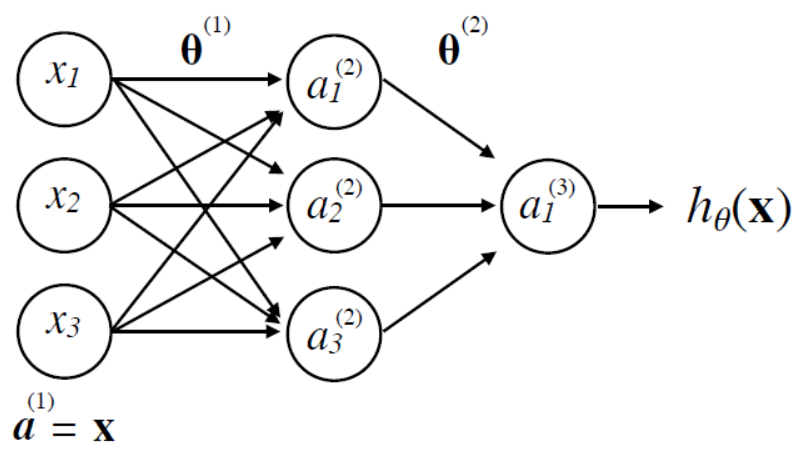
\includegraphics[width=0.5\textwidth]{images/NeuralNetworks3.png} \\ \\
    \end{tabular}
\end{center}
Node $a_1^{(2)}$ takes as input the three outputs of the first layer and through the nonlinear function $f$ calculates the linear combination of the three inputs plus the bias:
\begin{equation} \tag*{}
    a_1^{(2)} = f(\theta_{10}^(1)x_0 + \theta_{11}^(1)x_1 + \theta_{12}^(1)x_2 + \theta_{13}^(1)x_3)
\end{equation}
This is done for all nodes in the layer.
$\theta^{(j)}$ denotes the matrix of weights between layer $j$ and $j+1$.
The summation of all linear combinations of a layer is denoted by the letter $z_i^{(j)}$ where $j$ denotes the number of the layer, in this case $a_1^{(2)} = f(z_1^{(2)})$.
If we focus only on the last hidden layer we can see that what we do is the same as logistic regression in which the function $h_\theta(x) =f(\theta^{(2)}a^{(2)})$ and the input is no longer the features but is the $a^{(2)}$ learned from the network.
This makes us realize that all the previous hidden layers do is learn latent features from the data.

\subsection{Boolean Functions}
Neural networks can model various logic functions; a single perceptron can model a wide range of logic functions.
But the XOR function is not learnable by a perceptron.
The solution to this problem was the creation of deep neural networks multilayer. \\ \\
To represent an XOR function one must be able to solve a nonlinear classification problem, and to do this one must combine several perceptrons together in the following way:
\begin{center}
    \begin{tabular}{c}
        \\ 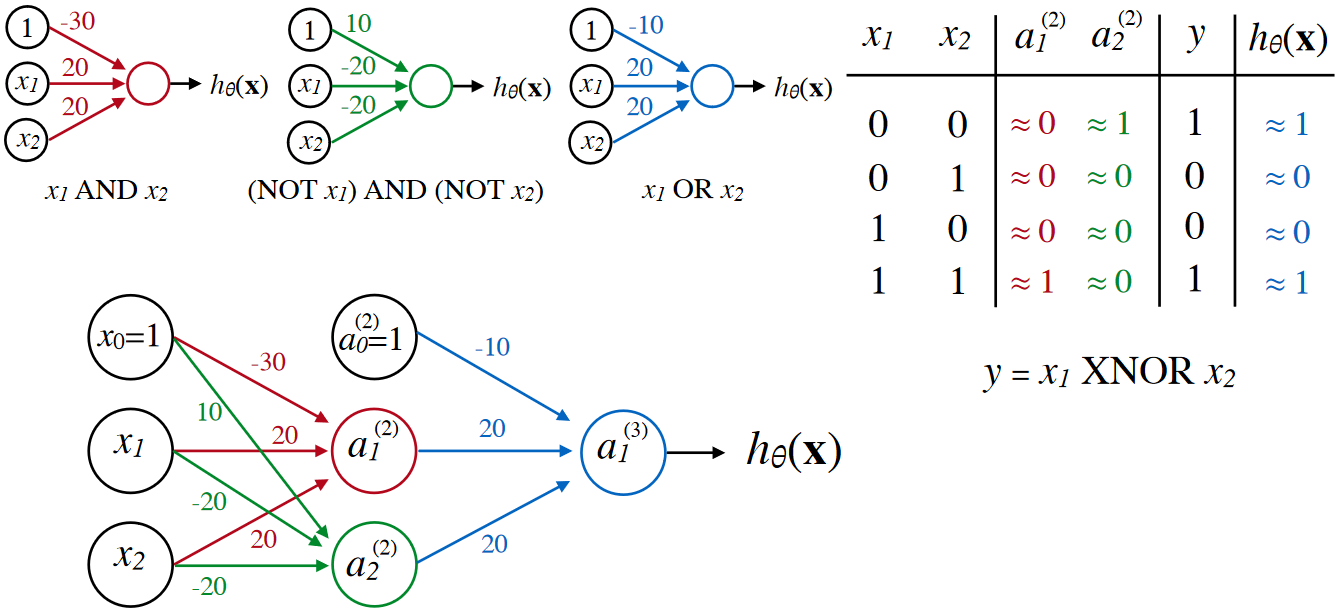
\includegraphics[width=0.9\textwidth]{images/NeuralNetworks4.png} \\ \\
    \end{tabular}
\end{center}

\subsection{Multiple Classes}
We can use two strategies to tackle a K-way multiclass classification problems:
\begin{itemize}
    \item \textbf{One-vs-one:}
    \begin{itemize}
        \item we train $K(K-1)/2$ binary classifiers
        \item each binary classifier is trained to discriminate between two classes
        \item at prediction time we apply a voting scheme
    \end{itemize}
    \item \textbf{One-vs-all:}
    \begin{itemize}
        \item we train a classifier per class
        \item each binary classifier is trained using its positive samples and samples belonging to all other classes as negative
        \item this strategy requires each classifier to produce a real-valued confidence score for its decision
        \item at prediction time we select the classifier with the highest confidence score
    \end{itemize}
\end{itemize}

\subsubsection{Loss Function}
The Loss Function for the logistic regression is:
\begin{equation} \tag{Loss Function}
    J(\theta) = -\frac{1}{m} \left[ \sum_{i=1}^m y_i \cdot \log(h_\theta(x_i)) + (1-y_i)) \cdot \log(1-h_\theta(x_i)) \right] + \frac{\lambda}{2m} \sum_{j=1}^n \theta_j^2
\end{equation}
To adapt it to multiclass classification, a summation is added to calculate the cost for the right class.  Since the class vector uses one hot encoding the cost is calculated only for the predicted class.
\begin{equation} \tag{Softmax}
    J(\theta) = -\frac{1}{m} \left[ \sum_{i=1}^m \sum_{k=1}^K y_k^{(i)} \cdot \log(h_\theta(x_i))_k + (1-y_k^{(i)})) \cdot \log(1-h_\theta(x_i))_k \right] + \frac{\lambda}{2m} \sum_{l=1}^{L-1} \sum_{i=1}^{u_l} \sum_{j=1}^{u_{l+1}} (\theta_{ji}^l)^2
\end{equation}
where:
\begin{itemize}
    \item $L$ is the number of layers in the network
    \item $u_l$ is the number of units in the layer $l$
\end{itemize}

\newpage